\documentclass{beamer}
\usepackage[utf8]{inputenc}
\usepackage[T1]{fontenc}
\usetheme{Madrid}  % Izberite stil teme
\usecolortheme{beaver}  % Izberite stil barve


% Nastavitve za naslovno stran
\title{Uporaba metode Monte Carlo}
\subtitle{Izračun števila $\pi$}
\author{Tomaž Travnikar}
\institute{Univerza v Ljubljani Fakulteta za strojništvo}
\date{\today}

\AtBeginSection[]
{
  \begin{frame}
    \frametitle{Kazalo}
    \tableofcontents[currentsection]
  \end{frame}
}

\AtBeginSubsection[]
{
  \begin{frame}
    \frametitle{Kazalo}
    \tableofcontents[currentsection,currentsubsection]
  end{frame}
}

\begin{document}

% Naslovna stran
\begin{frame}
  \centering
  
\includegraphics[width=3cm]{ULFS_logotip.jpg} % Dodajte ime datoteke za svoj logotip
  \vspace{1cm} % Dodajte želen vertikalni razmik
  \titlepage
\end{frame}

% Preostanek predstavitve tukaj
% Kazalo
\begin{frame}
  \frametitle{Kazalo}
  \tableofcontents
\end{frame}

% Preostanek predstavitve tukaj
\section{Teoretično ozadje}
\begin{frame}
  \frametitle{Metoda Monte Carlo}
  Metoda Monte Carlo je deterministična simulacijska metoda ali algoritm, ki s pomočjo naključnih ali kvazinaključnih števil in velikega števila izračunov in ponavljanja omogočajo predvidevanje obnašanja zapletenih matematičnih sistemov.
  \pause

  
  S pomočjo te metodo bomo izračunali približno vrednost števila pi. To storimo tako, da primerjamo ploščini kvadrata in njemu včrtanega kroga. Ploščino ocenimo tako, da generiramo veliko število naključnih točk, potem pa preverimo, ali se te nahajajo v krogu , ali zunaj njega.
  \end{frame}
  
\begin{frame}
  \frametitle{Osnovna enačba}
  Enačba za izračun π:
  \begin{equation}
    \pi = 4 \cdot \left(\frac{A_{\text{kroga}}}{A_{\text{kvadrata}}}\right)
  \end{equation}
  kjer je:
  \begin{align*}
    A_{\text{kroga}} &= \text{Površina kroga} \\
    A_{\text{kvadrata}} &= \text{Površina kvadrata}
  \end{align*}
\end{frame}

\begin{frame}
  \frametitle{Enačba za aproksimacijo π}
  Enačba za izračun $\pi$ je lahko zapisana kot:
  \begin{equation}
    \pi \approx 4 \cdot \left(\frac{N_{\text{krog}}}{N_{\text{kvadrat}}}\right)
  \end{equation}
  kjer veljata naslednji definiciji:
  \begin{align*}
    N_{\text{krog}} &\text{ - Število točk znotraj kroga} \\
    N_{\text{kvadrat}} &\text{ - Število vseh točk}
  \end{align*}
\end{frame}

\section{Reševanje v Matlabu}
\begin{frame}
  \frametitle{Vrednost približka}
  V programskem okolju Matlab sem napisal kodo, ki aproksimira število $\pi$,
  po metodi Monte Carlo. Za izračun približka sem uporabil 20000 točk. Rezultat je prikazan na sliki.
   \begin{figure}
    \centering
    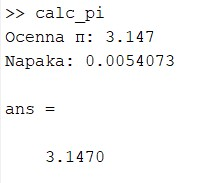
\includegraphics[width=0.3\textwidth]{Izgod.jpg}
    \caption{Izračunana vrednost števila $\pi$ in odstopanje od točne vrednosti}
  \end{figure}
\end{frame}
\section{Vizualizacija}
\begin{frame}
  \frametitle{Vizualizacija}
  Izrisal sem vse točke in označil posamezna območja.
  \begin{figure}
    \centering
    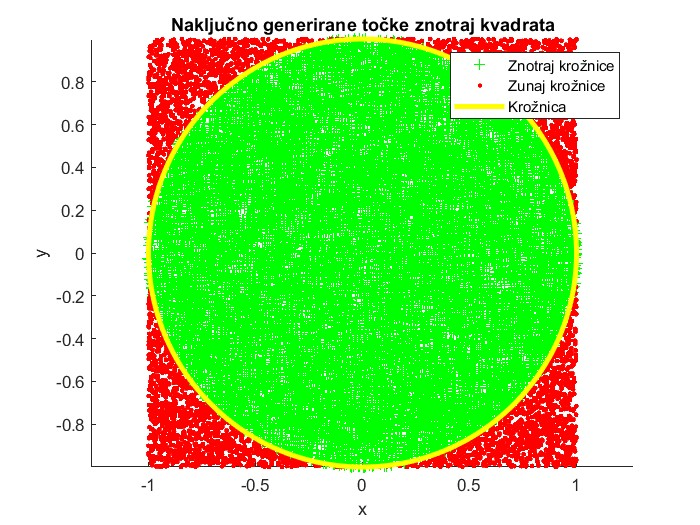
\includegraphics[width=0.6\textwidth]{Graf.jpg}
    \caption{Vizualizacija naključnih točk}
  \end{figure}
\end{frame}
\begin{frame}
  \frametitle{Viri}
  
  \begin{thebibliography}{1} % Uporabite največje število virov, ki jih boste citirali
    \bibitem{ime:vir} Marko Jereb. "Monte Carlo metoda - skupek računalniških algoritmov za reševanje numeričnih problemov z uporabo naključnega izbiranje." Lokar.fmf. 22.10.2023. \url{https://lokar.fmf.uni-lj.si/www/rom_konferenca/konferenca_2016/Monte_Carlo_metoda.html}.
  \end{thebibliography}
\end{frame}

\end{document}